\documentclass[a4paper,12pt,oneside]{ThesisStyle}
\usepackage[utf8]{inputenc}
\usepackage{thesis-style-summary}
\usepackage[english]{babel}

\begin{document}

\frontmatter

\pagenumbering{gobble}

\hypersetup{pageanchor=false}
\begin{titlepage}

  % Upper part of the page
  
\includegraphics[scale=0.9]{img/logo_eps.png} \\[1cm]
  \begin{center}
    \textsc{\Large Master's Thesis} \\[1cm]

    % Title
    \begin{spacing}{2}
      \HRule \\
      \textbf{\Huge Tuning a Generative Language Model for the Creation of Customized Chatbots for Public Administrations} \\
      \HRule \\[0.5cm]
    \end{spacing}

    % Author and supervisor and other data
    {
    \large
    \emph{Author:} \\
    Martí \textsc{Mas Fullana} \\[1cm]
    Setembre 2024 \\[1cm]
    Master's in Data Science \\[1cm]
    \emph{Supervisor:} \\
    Josep \textsc{Suy Franch} \\
    }

  \end{center}
\end{titlepage}
\hypersetup{pageanchor=true}

\titlepage

%\dominitoc

\pagenumbering{roman}

\mainmatter

\chapter{Summary}
\label{cap:summary}

\section{Introduction}
\label{sec:introduction}

This master's thesis explores the development of a customized chatbot system using GPT (Generative Pre-trained Transformer) and RAG (Retrieval Augmented Generation) technologies to improve the efficiency of public administration services in Catalonia, specifically targeting social rights and benefits. The project, conducted in collaboration with DXC Technology, focuses on creating a multilingual, accessible, and user-friendly interface while optimizing the chatbot's performance in terms of accuracy and cost.

Key components of the system include:

\begin{itemize}
    \item \textbf{Frontend Interface:} Built with Angular to handle user interactions.
    \item \textbf{Backend System:} Manages the conversation flow, connects with Azure services, and employs a Vector Search API for information retrieval.
    \item \textbf{Data Preparation:} Involves sourcing information from public websites and processing it to improve chatbot responses.
\end{itemize}

\section{Background}
\label{sec:background}

The thesis delves into the evolution of dialogue systems from rule-based models to advanced AI-driven systems. Key technologies and methods employed in this project include:

\begin{itemize}
    \item \textbf{Generative Pre-trained Transformer (GPT):} A series of models from GPT-1 to GPT-4o that progressively improved natural language processing capabilities.
    \item \textbf{Retrieval Augmented Generation (RAG):} Integrates database retrieval with generative models to enhance response accuracy and relevance.
\end{itemize}

These technologies help in developing chatbots that are contextually aware and capable of providing precise information based on user queries.

\section{Objectives}
\label{sec:objectives}

The main objective is to develop an advanced chatbot using GPT and RAG technologies that can provide accurate responses based on a database of social rights and benefits in Catalonia. The specific goals are:

\begin{itemize}
    \item \textbf{Model Selection:} Choose an appropriate GPT model.
    \item \textbf{RAG Integration:} Implement a retrieval system for precise information access.
    \item \textbf{User Experience:} Design an accessible and user-friendly interface.
    \item \textbf{Evaluation and Validation:} Conduct user testing and performance analysis.
\end{itemize}

\section{Methodology}
\label{sec:methodology}

The project employs the SCRUM methodology, an agile framework that supports iterative and incremental progress, ensuring adaptability and collaboration. Key roles and practices include:

\begin{itemize}
    \item \textbf{SCRUM Roles:} Product Owner, SCRUM Master, Development Team.
    \item \textbf{Sprint Planning:} Organizes the workload in two-week cycles.
    \item \textbf{Daily Stand-ups:} Maintain team communication and transparency.
    \item \textbf{Sprint Review and Retrospective:} Collect feedback and continuously improve the process.
\end{itemize}

Data is collected and prepared from public websites, which is then indexed into a PostgreSQL database (with the PGVector plugin enabled) using the LlamaIndex Python library to facilitate efficient information retrieval.

\section{Architecture}
\label{sec:architecture}

\begin{figure}[h]
  \centering
  \includegraphics[width=0.8\textwidth]{img/Full DSO App Architecture.drawio.png}
  \caption{App Architecture}
  \label{fig:architecture}
\end{figure}

The chatbot system's architecture consists of several components:

\begin{itemize}
    \item \textbf{Frontend:} Built with Angular, this handles the user interface, voice input, and interaction management.
    \item \textbf{Backend:} Manages the conversation flow, error handling, and integrates with external services.
    \item \textbf{Azure Services:} Utilized for Speech-to-Text and Text-to-Speech functionalities.
    \item \textbf{Vector Search API:} A custom component for information retrieval that enhances response accuracy.
\end{itemize}

The system uses a modular design, enabling easy adaptation for future applications. The chatbot's top-level flow diagram is shown in Figure \ref{fig:coversation_process}. Figure \ref{fig:architecture} illustrates the app architecture.

\begin{figure}[h]
    \centering
    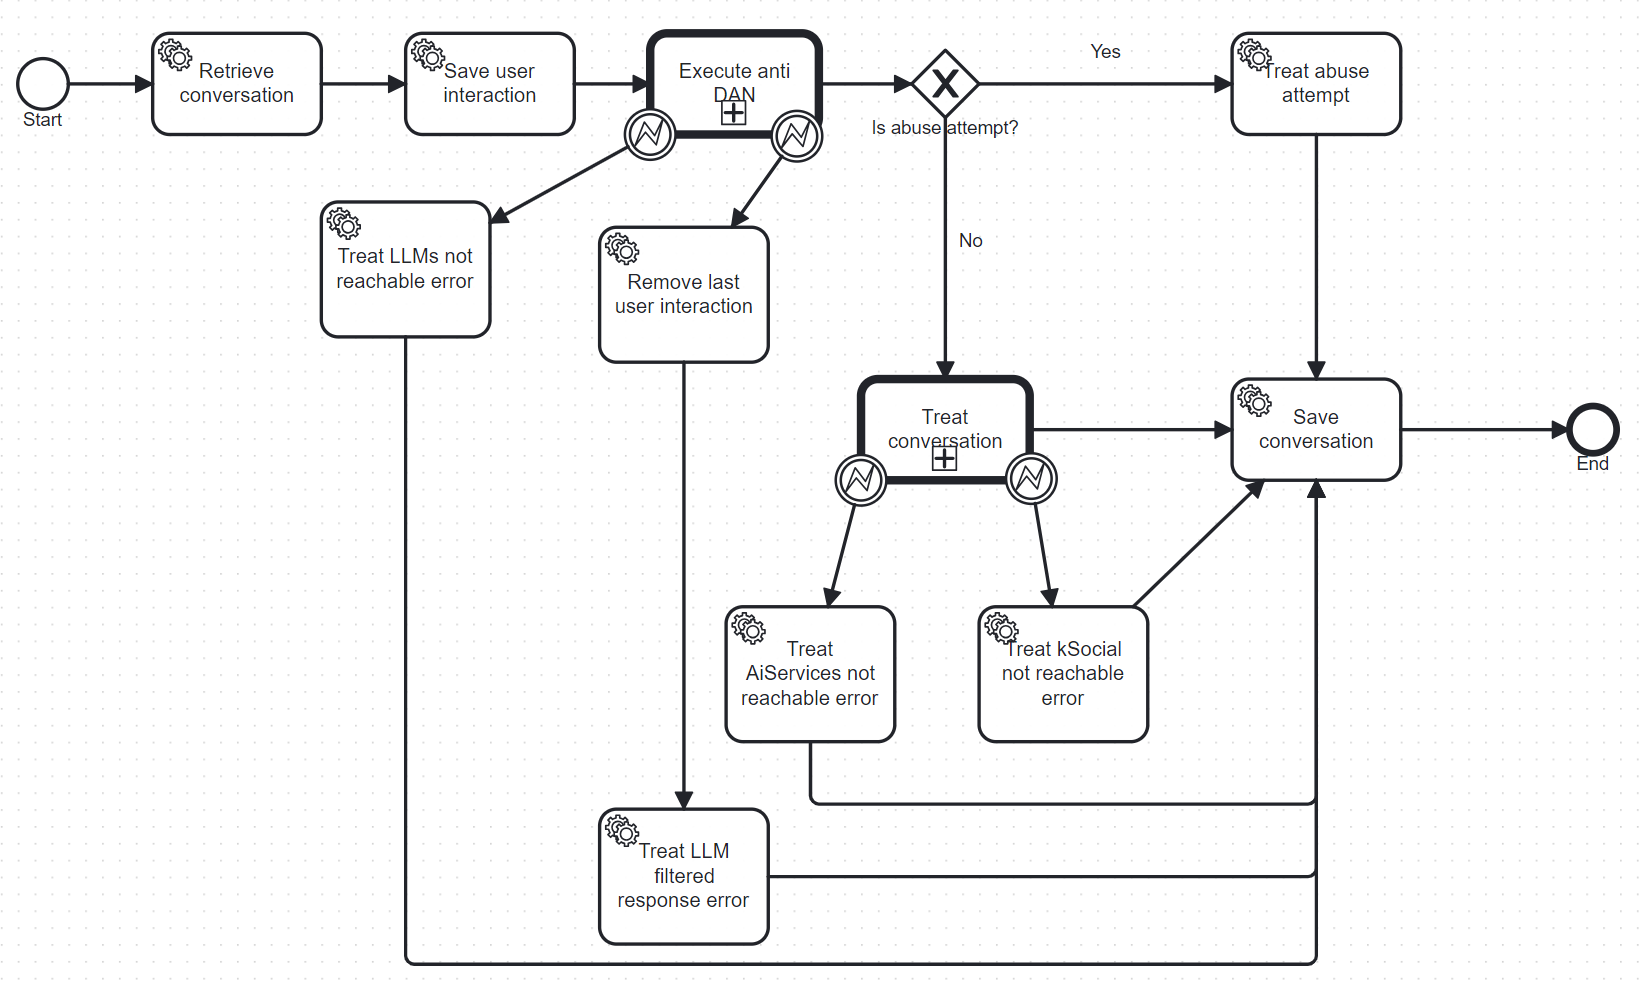
\includegraphics[width=0.7\textwidth]{img/Conversation_process.bpmn20.png}
    \caption{Top level chatbot flow diagram}
    \label{fig:coversation_process}
\end{figure}

\section{Results}
\label{sec:results}

The performance of the chatbot was evaluated using a benchmark of 35 questions, comparing the standard RAG and Small to Big Retrieval (STBR) methods. The STBR method demonstrated superior accuracy (0.79 average) compared to the standard RAG method (0.65 average), with a more consistent performance across different queries. However, STBR requires more computational resources, making it suitable for scenarios where accuracy is prioritized over speed.

\begin{table}[H]
  \centering
  \begin{tabular}{|c|c|c|}
    \hline
    \textbf{Method} & \textbf{Accuracy \(\uparrow\)} & \textbf{Standard Deviation \(\downarrow\)} \\
    \hline
    Normal RAG      & 0.65                           & 0.031                                      \\
    STBR RAG        & \textbf{0.79}                  & \textbf{0.024}                             \\       
    \hline
  \end{tabular}
  \caption{Results of the benchmark. In bold we show the best result.}
  \label{tab:benchmark_results}
\end{table}

\section{Conclusions}
\label{sec:conclusions}

The project successfully developed a chatbot system that enhances the delivery of social rights and benefits information to users in Catalonia. The system's modular architecture, combined with advanced language models, provides a flexible and scalable solution for public administration needs. The use of RAG technology significantly improves the accuracy and relevance of the chatbot's responses.

\section{Future Work}
\label{sec:future_work}

Future enhancements could include:

\begin{itemize}
    \item \textbf{Multilingual Support:} Extend the system to support additional languages.
    \item \textbf{Enhanced Accessibility:} Improve features for users with disabilities.
    \item \textbf{Performance Optimization:} Reduce response times and improve scalability.
    \item \textbf{Continuous Improvement:} Regular user testing and iterative development.
\end{itemize}

\end{document}
